\documentclass[11pt,a4paper]{article}

\usepackage[margin=1.8cm]{geometry}
\usepackage{pdflscape}
\usepackage[T1]{fontenc}
\usepackage[utf8]{inputenc}
\usepackage{lmodern}
\usepackage{microtype}
\usepackage{graphicx}
\usepackage{booktabs}
\usepackage{tabularx}
\usepackage{array}
\usepackage{fancyhdr}
\usepackage{caption}
\usepackage[hidelinks]{hyperref}

\setlength{\parindent}{0pt}
\setlength{\parskip}{5pt}
\pagestyle{fancy}
\fancyhf{}
\lhead{MLOps GBFS Bike-Sharing}
\rhead{Laporan Eksperimen MLflow}
\cfoot{\thepage}
\setlength{\headheight}{14pt}
\renewcommand{\headrulewidth}{0.4pt}
\renewcommand{\footrulewidth}{0pt}
\captionsetup{font=small,labelfont=bf}

\begin{document}

\begin{center}
  {\LARGE\bfseries Laporan Training dan Tracking MLflow}\par
  \vspace{4pt}
  MLOps GBFS Bike-Sharing\par
  22 Oktober 2026
\end{center}

\section*{Tujuan}
Tujuan training adalah membandingkan tiga konfigurasi model Random Forest untuk
memprediksi jumlah sepeda tersedia dan dock kosong per stasiun, 30 menit ke
depan. MLflow mencatat parameter, metrik, dan model pada setiap run.

\section*{Sumber data dan preprocessing}
Data berasal dari artifact GitHub Actions run
\href{https://github.com/Zeropeepo/MLOps-GBFS-Bike-Sharing/actions/runs/39779055751}{\texttt{39779055751}}
di branch \texttt{main}. Artifact tersebut memuat pasangan feed GBFS yang
diambil pada pukul 12:31 UTC tanggal 22 Oktober 2026. Snapshot dan manifest ditambahkan ke
repository lokal, kemudian feature table dibangun ulang.

\begin{itemize}
  \item Feature table: 32.270 baris, termasuk 9.936 baris dengan kedua target
        30 menit tersedia.
  \item Data berlabel bertambah 2.484 baris dibanding versi sebelumnya.
  \item DVC pointer diperbarui; \texttt{dvc status} menyatakan data up to date.
\end{itemize}

\section*{Hasil eksperimen}
Data dibagi secara kronologis tanpa shuffling: 7.452 baris untuk training dan
2.484 baris untuk validation. Pemilihan model menggunakan mean RMSE dari kedua
target; nilai lebih rendah lebih baik.

\small
\begin{tabularx}{\textwidth}{@{}l>{\raggedright\arraybackslash}Xrrrrr@{}}
\toprule
Run & \shortstack[l]{Parameter\\(estimators / depth / leaf)}
& Bikes MAE & Bikes RMSE & Docks MAE & Docks RMSE & Mean RMSE \\
\midrule
RF1 & 100 / 10 / 2 & 2.0237 & 3.7317 & 2.0156 & 3.6008 & 3.6663 \\
RF2 & 200 / 16 / 2 & \textbf{1.7105} & \textbf{3.4491} & \textbf{1.6799}
& \textbf{3.3028} & \textbf{3.3760} \\
RF3 & 300 / tanpa batas / 4 & 2.0782 & 4.0190 & 2.0544 & 3.9147 & 3.9669 \\
\bottomrule
\end{tabularx}
\normalsize

\section*{Metadata model terbaik}
\begin{tabularx}{\textwidth}{@{}>{\bfseries}lX@{}}
Registry & \texttt{GBFSBikeAvailabilityRegressor}, versi 3, status \texttt{READY} \\
Run ID & \texttt{7a1a6c9ab27a44378c36b69a6072f9e3} \\
Parameter & \texttt{n\_estimators=200}, \texttt{max\_depth=16},
             \texttt{min\_samples\_leaf=2}, \texttt{random\_state=42} \\
Validation & Bikes RMSE 3.4491, R\textsuperscript{2} 0.9240;
             docks RMSE 3.3028, R\textsuperscript{2} 0.9362 \\
Mean RMSE & 3.3760 \\
\end{tabularx}

Model ini merupakan kandidat terbaik dari tiga konfigurasi yang diuji.
Validation hanya mencakup satu kelompok waktu observasi terbaru, sehingga hasil
ini masih bersifat awal dan belum menjadi klaim kesiapan deployment.

\clearpage
\begin{landscape}
\thispagestyle{empty}
\section*{Bukti MLflow UI: parameter run}
\begin{center}
  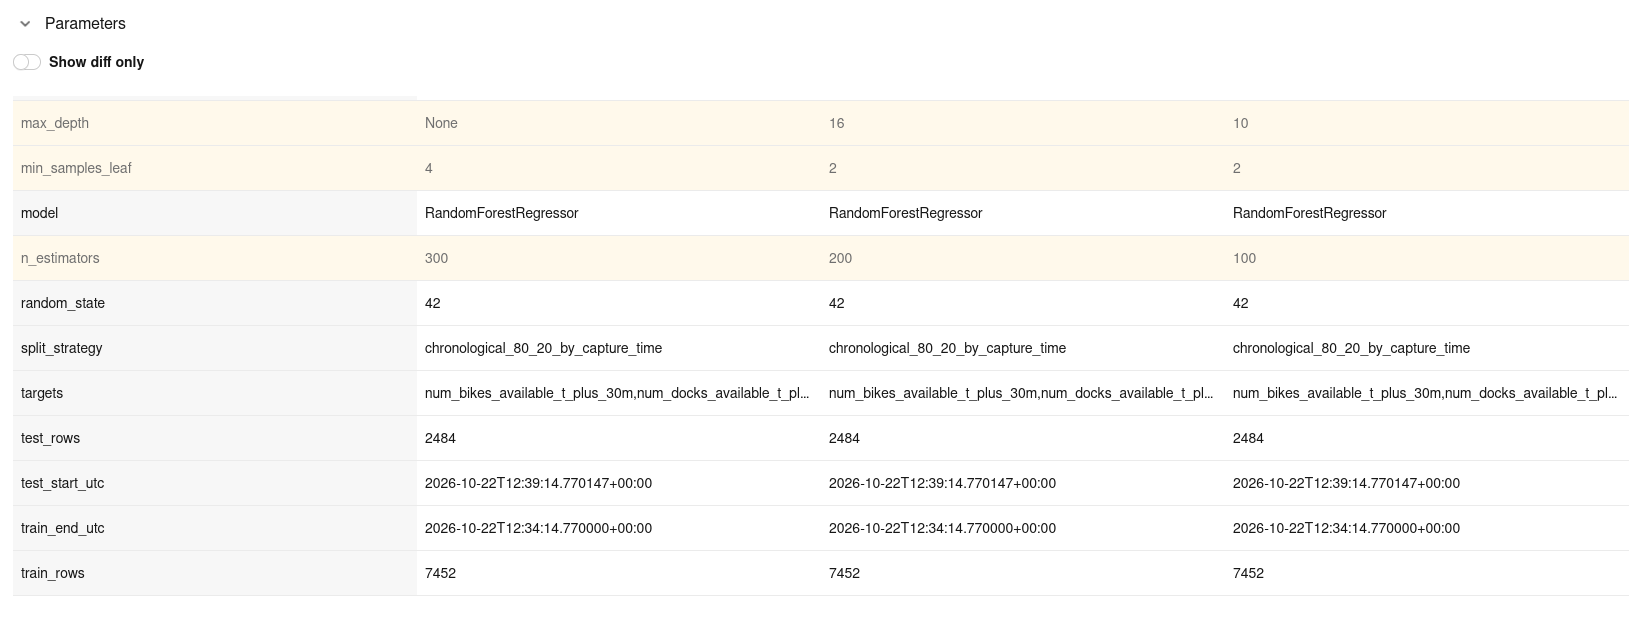
\includegraphics[width=0.98\linewidth,height=0.76\textheight,keepaspectratio]
    {mlflow_screenshots/Screenshot_2026-10-22-213843.png}
  \captionof{figure}{Perbandingan parameter tiga run pada MLflow UI.}
\end{center}
\end{landscape}

\clearpage
\begin{landscape}
\thispagestyle{empty}
\section*{Bukti MLflow UI: metrik}
\begin{center}
  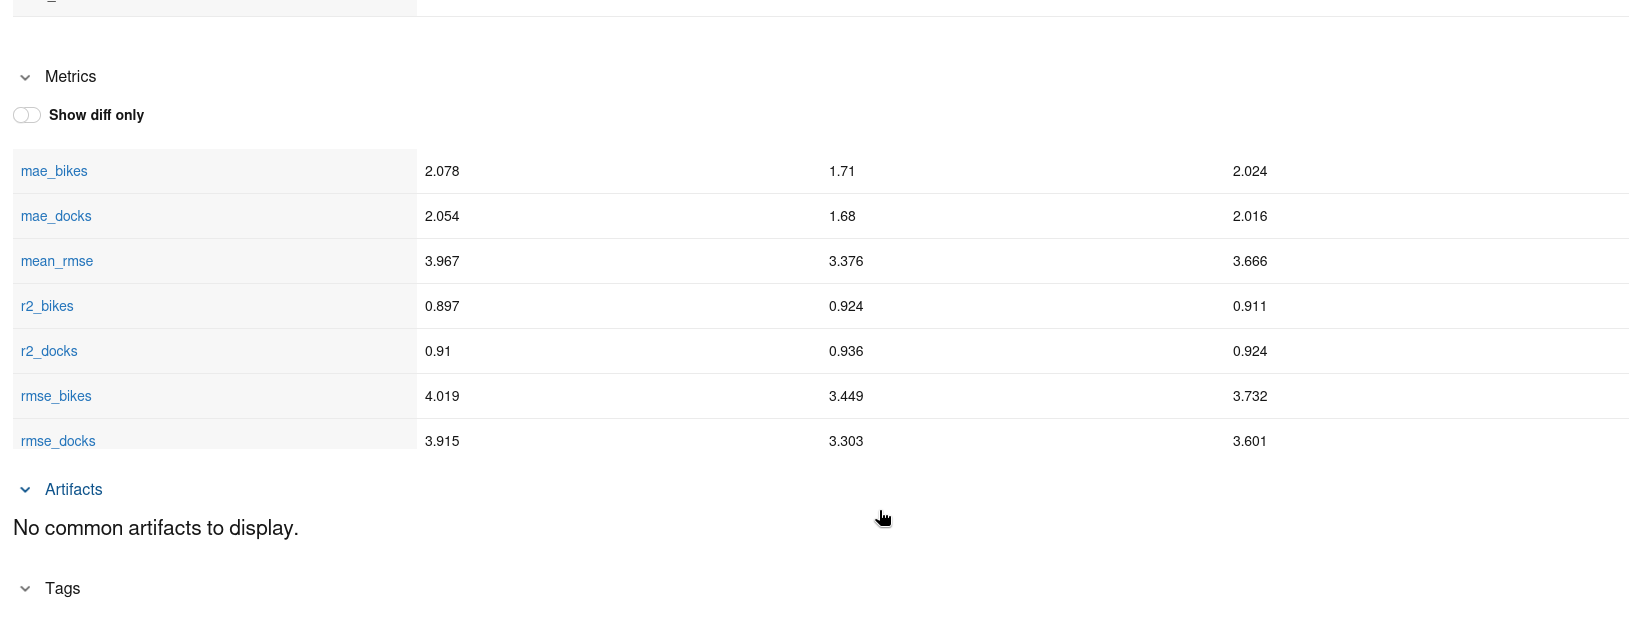
\includegraphics[width=0.98\linewidth,height=0.76\textheight,keepaspectratio]
    {mlflow_screenshots/Screenshot_2026-10-22-214025.png}
  \captionof{figure}{Perbandingan metrik MAE, RMSE, R\textsuperscript{2}, dan mean RMSE.}
\end{center}
\end{landscape}

\clearpage
\begin{landscape}
\thispagestyle{empty}
\section*{Bukti MLflow UI: visualisasi perbandingan}
\begin{center}
  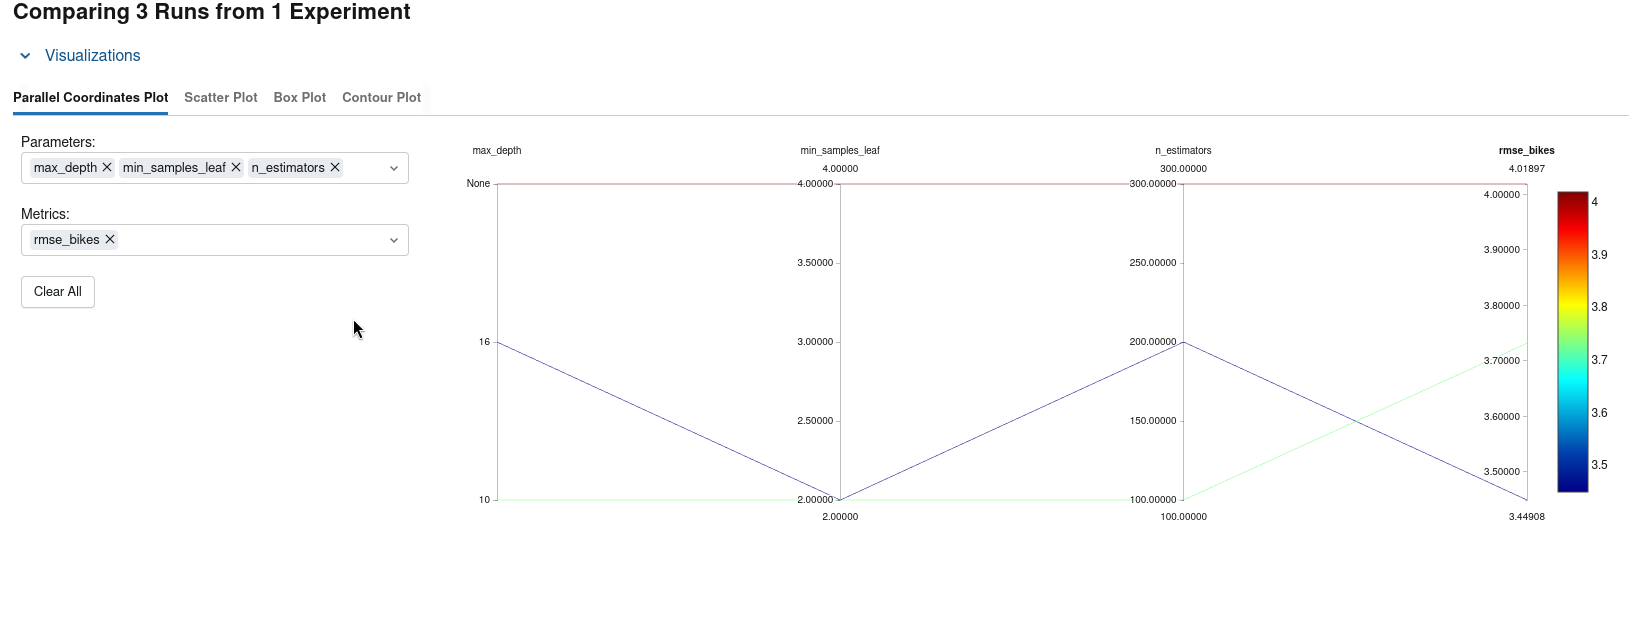
\includegraphics[width=0.98\linewidth,height=0.76\textheight,keepaspectratio]
    {mlflow_screenshots/Screenshot_2026-10-22-214359.png}
  \captionof{figure}{Parallel Coordinates Plot untuk tiga run; warna menunjukkan
  nilai \texttt{rmse\_bikes}.}
\end{center}
\end{landscape}

\end{document}
